\newpage
\subsection{Implementation of the embedded server}
Here will be STM32 server implementation.







 One solution is to use closed encrypted proprietary
protocol and be calm, but as it was mentioned earlier, it limits the possibility of integration
between other embedded systems. It this case all of your devices should support
that protocol and you choise of different hardware is limited. Proprietary
protocols are often vendor-specific, code is closed, documentation is not free
and all it works only with the proprietary devices from the manufacturer.


\begin{center}
 \begin{figure}[h]
	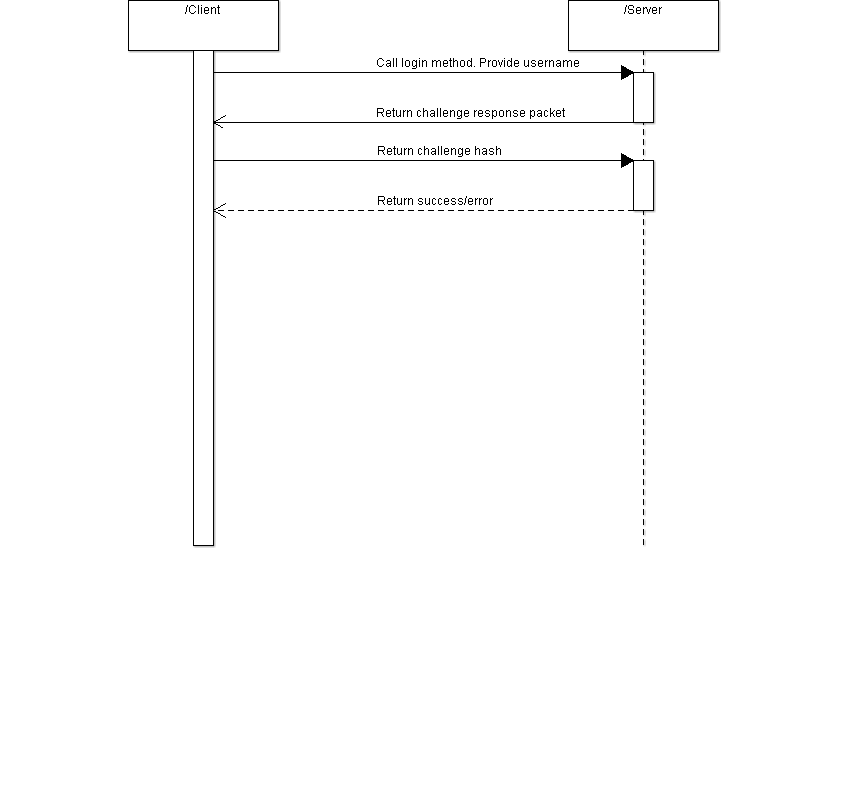
\includegraphics[width=\textwidth]{../images/implementation/embedded_server/SequenceDiagram.png}
	\caption{Client authentification process}
	\label{fig:embedded_server_login_auth}
 \end{figure}
\end{center}


reversably encrypted form.

